%\addcontentsline{toc}{chapter}{Development Process}
\chapter{Design}

In FDD, large, detailed design documents are not necessary. A simple overview of desired features and a breakdown of the overall system are sufficient, and are what will be detailed in this chapter.

\section{Overall Architecture}
\label{sec:des_Architecture}
As the project was developed using Feature Driven Development (FDD), the initial design of the system focused on the desired features of the system. These features were:
\begin{enumerate} %Number these so they can be referenced later
	\item Download the dataset.
	\item Parse the original data into a more useful format.
	\item Allow a user to annotate the data with sentiment, to generate training and testing datasets.
	\item Train an AI algorithm on the datasets generated.
	\item Search the parsed data to find speech about a certain topic, or by a particular Member of Parliament.
	\item Use the trained AI algorithm to extract sentiment from the speech found.
	\item Display a comparison of the sentiment expressed about a topic or by an MP over time.
\end{enumerate}

Using these features, the overall system can be designed, and an unofficial class diagram can be created that can help guide implementation.

\begin{figure}[ht]
	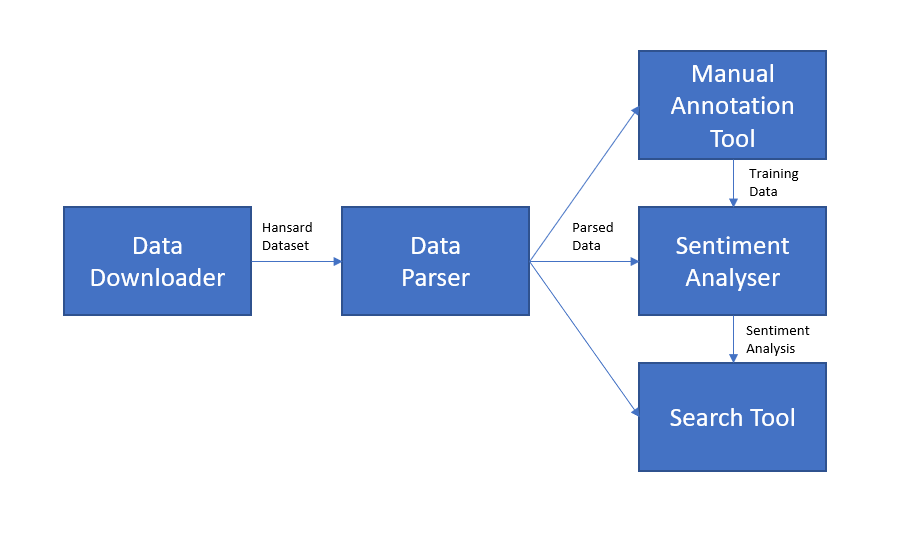
\includegraphics[width=\textwidth]{project_block_diagram}
	\caption{Functional block diagram of the overall system. Arrows represents data movement}
	\label{fig:project_block_diagram}
\end{figure}

As seen in Figure \ref{fig:project_block_diagram}, the system is broken down into functional blocks, each representing a distinct part of the system. They were split this way to maintain readability in the source code. Whilst it would have been possible to keep all functionality in a single file, it would have made maintaining the code very difficult. Each functional block is therefore a separate class in the Python source code, so any interaction between them is easy to manage.

\subsection{Data Downloader}
\label{sec:des_data_downloader}
The Data Downloader is designed to download all of the Hansard Dataset from the site on-line, and store it locally for use by the rest of the system. It is likely that this first block will only need to be run a single time, but still proves useful in ensuring all the data is downloaded.

The files are to be downloaded from the \href{http://www.hansard-archive.parliament.uk}{Hansard Archive} page. Each of the six series has a subdirectory under that root page, that contain all the data files. The data files have a distinct naming pattern that can be referenced using something like Regular Expressions in order to automate the downloading and searching of the files.

Originally, this was not going to be a part of the main system, as it is possible to download the data manually. However, only ten files are displayed on the web page each time, and some of the series have up to a thousand files to download. This can be seen in Figure \ref{fig:Archive_Screenshot}. Therefore, an automated downloader needs to be implemented that can download the data automatically. The Design should allow the user to select which series they want to download and where it should be saved, and then it should automatically connect to the web page and attempt to download all the files.

\begin{figure}[ht]
	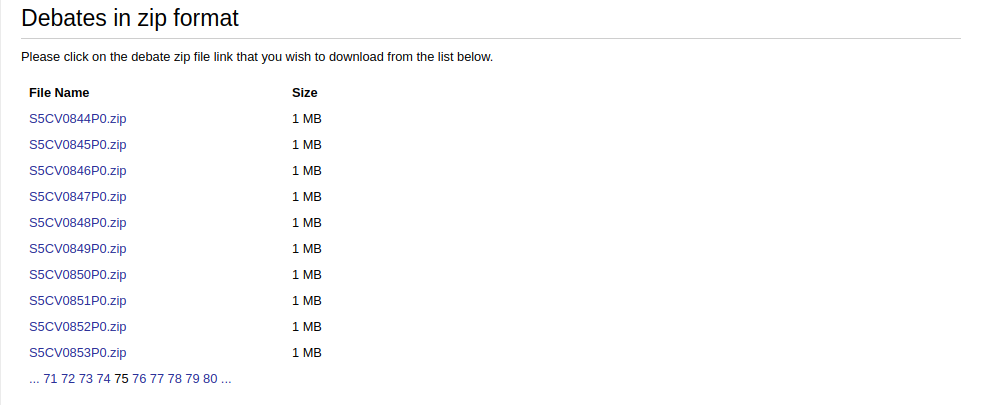
\includegraphics[width=\textwidth]{archive_screenshot}
	\caption{Screen capture from the Hansard Archive website, showing the number of files available}
	\label{fig:Archive_Screenshot}
\end{figure}

\subsection{Data Parser}
\label{sec:des_data_parser}
The Parser is designed to read the original files downloaded by the Data Downloader, and save all relevant data in separate location, in a more consistent layout than that of the original dataset. This should allow any usage of the data from other parts of the system to be much simpler, and thus faster and less prone to error. It should ensure speech is always attributed to the correct person, even if their names are presented differently. This means the Data Parser will have to utilize a part of NLP known as Name Disambiguation, which is not a simple task, and is discussed in further detail in Section \ref{sec:imp_name_disamb}.

Additionally, it was decided early on during the design that only Spoken speech would be used in this project. This was because written words were expected to be less likely to express any strong sentiment, as the written word gives the Member of Parliament time to edit and decide upon exactly what they wanted to respond to a question with. The spoken word was thought to be more likely to display the actual opinions and sentiments of the speaker, as they must respond in real time to questions and rebuttals.

\subsection{Manual Annotation Tool}
\label{sec:des_annotation_tool}
In Artificial Intelligence development, there is a concept known as \emph{Ground Truth}, which is a representation of the reality that an algorithm wants to predict; such as the changes to the stock market or the sentiment expressed by a piece of text. It's often commonly represented by the training data used to train an AI algorithm when using a supervised or semi-supervised algorithm. Thus, for this project, the ground truth must be decided upon and represented by a set of training and testing data.

The Manual Annotation Tool (the MAT) is designed to allow a user to create said testing and training datasets from the parsed data. It should show a selection of speech to the user, and ask them to annotate it as either a positive sentiment, negative sentiment, or neutral sentiment. These choices will be recorded, and can then be used to train a machine learning algorithm to extract sentiment from the remaining data. It would also provide the option to edit the text, the MP's name, or the topic title, to allow the user to correct typos transfered from the original dataset.

Originally, the MAT would display an entire paragraph of speech, displaying everything a Member of Parliament said about a topic on a particular day. However, this would often display too much text, with parts showing positive sentiment and other parts of the same text showing negative sentiment. Additionally it was realized that attempting to train an AI algorithm on these large blocks of text would be far too complex. For those reasons, the MAT was modified so that it would only display a single sentence at a time, allowing a more accurate way of annotating sentiment.

The MAT is designed to accept the parsed data from the parser described in Section \ref{sec:des_data_parser}, and should break the speech found in the data down into sentences, then output the sentence and sentiment annotated to it as described in Section \ref{sec:des_anotate_data}

\subsection{Sentiment Analyzer}
\label{sec:des_sentiment_analyzer}
The Sentiment Analyzer will use the datasets generated by the MAT and produce a model based off the data. It should also provide the ability to load a previously trained model, rather than spend time retraining every time the system is run. Once trained or loaded, it should be able to accept blocks of text, which it can then extract sentiment from, and return it.

As AI algorithms are trained on "Features" rather than plain text, the Sentiment Analyzer must have some method of converting a sentence or paragraph into a set of features for the algorithm to use. Following on from a tutorial by \emph{sentdex} \cite{NLTKYoutubePlaylist}, it appears that a good way to turn the text into a set of features is to use a dictionary, where the keys are the most common words from the training set, and the value is a True or False, for if the word is contained in the sentence or paragraph given. The potential issue with this is the loss of context, as separating the words completely will lose any negation, such as in the sentence "This is not good".

\subsection{Search Tool}
\label{sec:des_search_tool}
The Search Tool will be used by the user to search through the data for a particular Member of Parliament, to get their speech and its sentiment, or for a particular topic, to get the sentiment expressed about that topic.

The user would be presented with an option to search for either a Member of Parliament by name or a topic by title. It should then display the results of the search, showing examples of what was said about the topic, or if searching by MP, showing the topics they discussed and the things they said. It should also display an average sentiment expressed by that person or about that topic.

This average would have to be calculated in some way, likely by attributing a score of -1 for negative sentiment and +1 for positive sentiment. It would then likely be displayed using some sort of descriptive value rather than just the number; such as \emph{Neutral} for a score around the 0 mark, or \emph{Very Positive} for something close to 1.


\section{Data Design}
\label{sec:des_data}
As parts of the system were designed to modify the layout of the original data at times, the formatting of said data had to be designed as well.

\subsection{Parsed Data}
\label{sec:des_parsed_data}
The original Hansard Data was a set of XML files generated from the official Hansard Report. Some of the files referring to older reports, such as those from the 1800s, appear to have been scanned in using some form of Optical Character Recognition, and thus contained some slight errors in some of the text. This also means that the data is not structured as well as might be expected from XML data.

As can be seen in figure \ref{fig:S5_sample_screenshot}, the data files contain data that is not useful to the project. For instance, there are references to images that were not included as a part of the download, presumably a scan from the original written report, though this is not made clear. In addition, there are \emph{<p>} tags, representing paragraphs, which include ID numbers that are also not needed by this project.

\begin{figure}[ht]
	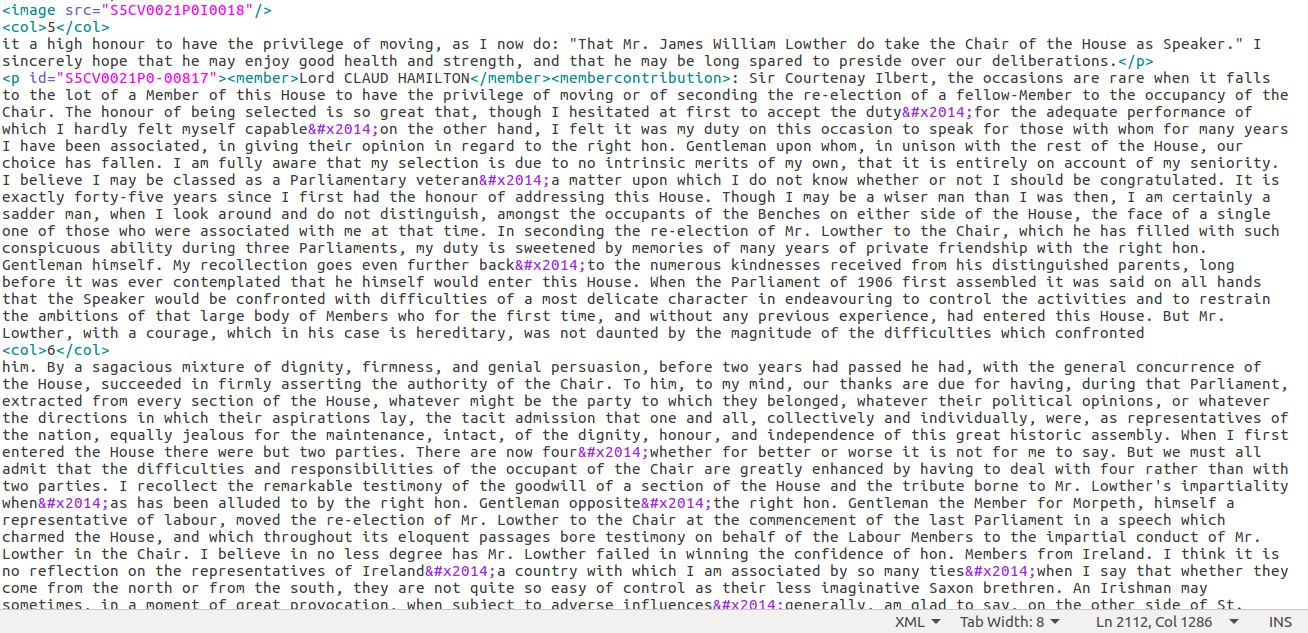
\includegraphics[width=\textwidth]{S5_sample_data}
	\caption{A sample of data from the file \emph{S5CV0021P0.xml}, a file from the fifth series of data}
	\label{fig:S5_sample_screenshot}
\end{figure}
For the parser, the format of the data files that it produces was originally designed as shown in Algorithm \ref{lst:parsed_data}.
\begin{lstlisting}[language=XML,
				   float=ht,
				   caption={Earlier version of the Parsed Data design},
				   label={lst:parsed_data}]
<date dateformat="1984/04/13">	
    <speech>
        <member>memberName</member>
        <topic>topicTitle</topic>
        <stance>POS/NEG</stance>
        "Actual Text of Speech would go Here"
    </speech>
    ....
</date>
....
\end{lstlisting}
The ellipses represent repeats, so inside the \emph{Date} tags, multiple \emph{speech} tags, all formatted like the one shown, can exist. A file may also contain multiple \emph{Date} tags. 

This, however, was causing some issues during development based around the size of the produced files, which were growing to thousands of lines long and several Gigabytes in size, as each entire series of data was being parsed into the same file. In order to combat the slow speeds of accessing such large files, and other issues caused by the layout, the data format was changed. Now, each unique date found within the source is saved in a separate file, and within this file the data was formatted in its final form.
Each date file is an XML file, the structure of which can be represented as a tree, shown in Figure \ref{fig:parsed_data_tree}.

\begin{figure}[ht]
	\includegraphics[width=\textwidth]{parsed_data_tree}
	\caption{Diagram showing the structure of the parsed data, in XML. The \emph{Date} tag is the root of the file}
	\label{fig:parsed_data_tree}
\end{figure}

Each file can contain multiple member tags, which each have the member of parliament’s name as an attribute. Each member tag can contain multiple tags for the topics they discuss, each of which have the topic title as an attribute. Each topic tag can have multiple speech tags, each speech tag containing the verbatim copy of what the member said about the particular topic.

\subsection{Annotated Data}
\label{sec:des_anotate_data}
The formatting of the annotated data files was also designed at this stage. It was decided that the files would be saved as CSV files (comma separated values), which is a simplistic database style where a line in the file represents a single record, each value of the record being separated by a comma, hence the name. The layout was designed as the following:

\textbf{Sentence, Sentiment, Member, Topic}

As shown, it was decided that the best way of annotating full speech was to split it by sentence, so that each sentence would be annotated with its own sentiment. This would simplify the training process for the machine learning algorithms, as it was thought that trying to train it on too large a block of text would result in sub par results, as these larger blocks of text can often express multiple sentiments interwoven into the speech. Attempting to train on, or even annotate, these larger more complicated blocks of speech would mean having to decide what the most important sentiment expressed would be, or work out the average sentiment. Due to this, any AI algorithm attempting to train on this would be training on data that expressed a varied sentiment, rather than a more polarized sentiment expressed in a single sentence. Of course, it is still possible that a single sentence might express positive sentiment towards one thing and simultaneously a negative sentiment towards something else, but dealing with these issues would take a lot more work than can be done on this project. 

\section{User Interface}
\label{sec:des_user_interface}
Due to the complexity of the project, it was decided that the system would only be interacted with via the command line. This meant that, beyond basic menus, no GUI had to be designed for use. It was though that, should there be time during or after the project development, a GUI could be designed which worked with the existing functions, but it was not considered system critical to have a GUI.

The search tool described in Section \ref{sec:des_search_tool} is designed to be the part used by most users, and so a mock up of the command line interface is shown in Figure \ref{fig:search_mockup}

\begin{figure}[ht]
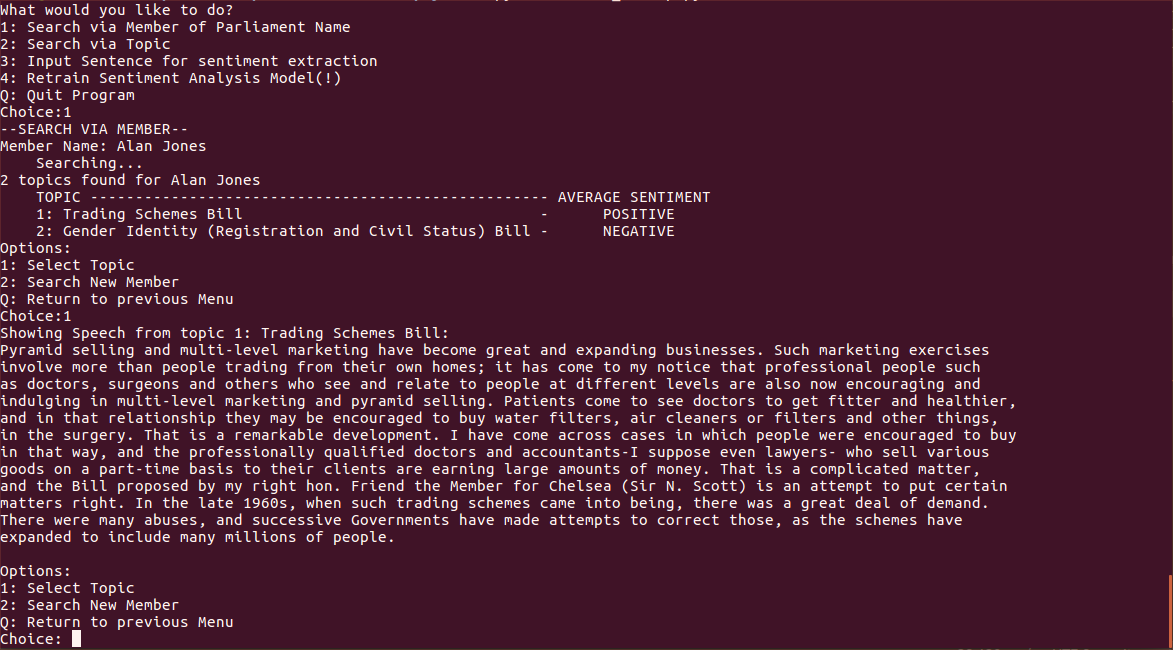
\includegraphics[width=\textwidth]{search_mockup}
\caption{A mockup design of the Search tool, which would be the main user interface for the project}
\label{fig:search_mockup}
\end{figure}

\section{Algorithm Design}
\label{sec:des_algorithm}

\subsection{AI Algorithm Choice}
\label{sec:des_AI_algorithm}
There are many potential algorithms that may be chosen for this project. It may prove difficult to choose one, or more, without simply trying them. The design calls for the use of Naive Bayes at first, mainly as its one provided by the NLTK package. However, multiple other algorithms may be tested, and the results compared to decide on the final choice. Should multiple algorithms prove useful, a voting system could be implemented, which applies each algorithm, and they cast a vote to what sentiment they calculate the text as. The votes would then be counted and the result shown.

\subsubsection{Naive Bayes}
Naives Bayes is a supervised algorithm with uses the statistical analysis of Bayes Theorem as to classify data. It treats each feature as completely distinct, which isn't accurate for NLP, but will may suffice for development of the system.

Bayes Theorem provides a way to calculate the probability of something occurring, for this project text being positive or negative, given it's prior probability, and the probability of it given the Data provided.\cite{Mitchell1997}. Text being classified as one thing or the other is usually called a \emph{Hypothesis} in this regard. The mathematical representation of Bayes Theorem can be seen in Figure \ref{fig:bayes_theorem}.
\begin{figure}[ht]
$$ P(h \mid D) = \frac{P(D \mid h) \, P(h)}{P(D)} $$
\caption{Bayes Theorem}
\label{fig:bayes_theorem}
\end{figure}

Where $P(h \mid D)$ is the probability of the Hypothesis (in the case of this assignment the prediction that a sentence is either Positive or Negative) holding true given the data provided. $P(D \mid h)$ is the probability that the data is true, given the hypothesis; and $P(h)$ and $P(D)$ are the probabilities of the Hypothesis and the Data respectfully.

$P(h)$ is usually called the \emph{Prior Probability} of the Hypothesis, and reflects any background knowledge about the chance that the hypothesis is correct. In this project, this is likely to represent any form of bias in the training data, in that the prior probability of text being classified as positive would be equal to the percentage of training data that is labeled positive.

The Naive Bayes Classifier uses Bayes Theorem in a learning step in which the various probabilities of a class, such as \emph{positive} or \emph{negative}, are estimated, given the different attributes or the data\cite{Mitchell1997}. These estimations correspond to the learned hypothesis, which is then applied to the new instances to classify them.

\subsection{Parsing}
\label{sec:des_Parsing_algorithm}
The Data Parser needs to find and extract useful speech from the original data. Though said data is somewhat disorganized, in that speech can exist down almost any route through the XML tree and occur at any level, there are exploitable patterns that the Parser can use to find as much speech as possible. The overall method is documented in the pseudo-code Algorithm \ref{lst:parser_pseudocode}:
\begin{lstlisting}[float=ht, caption={Data Parser Pseudo-code}, label={lst:parser_pseudocode}]
for EACH FILE
    for EACH DATE TAG
    	if(DATE_FILE FOR DATE EXISTS)
        	LOAD DATE_FILE CONTENTS INTO DATE_XML
    	else
        	CREATE FILE
        	CREATE DATE_XML
    	for EACH CONTRIBUTION in DATE_TAG
        	GET CONTRIBUTION PARENT_TAG
        	GET MEMBER NAME AS CHILD OF PARENT_TAG
        	GET TITLE AS SIBLING OF PARENT_TAG
        	GET SPEECH FROM CONTRIBUTION
        	if MEMBER HAS BEEN SEEN BEFORE in CURRENT DATE_FILE
        	    if TOPIC HAS BEEN DISCUSSED BY MEMBER BEFORE
        			ADD SPEECH TO TOPIC
        		else
        			CREATE NEW TOPIC
        			ADD SPEECH
        	else
        		CREATE NEW MEMBER TAG
        		ADD TOPIC TO MEMBER TAG
        		ADD SPEECH TO TOPIC
        	ADD SPEECH TO DATE_XML

    SAVE XML TO DATE_FILE (OVERWRITE)
\end{lstlisting}

This shows that, so long as the parser can find a tag in the source XML for the date, all other relevant information can be found in relation to the position of this date tag in the XML. It also shows the method of ensuring all speech by one Member of Parliament is correctly attributed to them, to avoid repeated mentions of the same MP in the same file.

\section{Conclusion}
Once the design of all the major parts of the project had been finalized, this report will now move on to the implementation section, to discuss how implementing these designs went, what became more difficult than expected and what, if anything, had to be changed, as FDD means that once a design is completed, it can still be modified and changed depending on implementation.